% ----------------------------------------------------------
% Background
% ----------------------------------------------------------
\chapter{Background}

\textcolor{red}{<<Presentation of the chapter with its contents>>}

\section{Design and Verification of Embedded Systems}

Embedded Systems and Systems-on-Chip (SoC) are in the center of the technological transformation of the modern world. The ubiquity of these systems can be endorsed by Internet-of-Things (IoT), Industry 4.0, and Smart Systems, to name a few examples. It reflects the rising complexity of these systems under different perceptions, such as power consumption, occupied area, scalability, and portability. In other words, it exposes an increasing demand for highly optimized systems, and therefore optimized processors. On the other hand, optimizing processors evidences an important concept of hardware design: Functional Safety. This is because the more optimizations in a system, the more prone to error the design process becomes. Consequently, methods for hardware design verification also need to improve.

In the last decades, methods for hardware design have been based mainly on Hardware Design Languages, such as VHDL and Verilog, at the Register Transfer Level (RTL) \cite{paper-pdd}. For most cases, the RTL design represents the reference model for the system, or “golden model”, and it is derived directly from specifications that are in most cases described in diagrams, or even in natural languages. Traditional techniques for verification of digital designs include simulation with test benches and assertions \cite{paper-symbolic}. Considering the mentioned increase on the complexity of processors and SoCs, these verification methods become more costly and time consuming. Writing test benches to cover the specified scenarios, running simulations and analysing wave forms are some examples of that. In addition, these techniques are also known as “bug hunting”, because they do not guarantee a bug free design. 

A higher-level description of the design, for instance the Electronic System Level (ESL), can be developed using programming languages like \textit{C++} associated with some special libraries such as \textit{SystemC}. Some advantages of ESL models are the rather faster simulations, achieved by modelling of communication as transactions instead of a cycle-accurate simulation, and well-established debugging tools. Furthermore, there are High-Level Synthesis (HLS) tools which allows these high-level descriptions to be used to generate the implementation of the design. Even though HSL tools have improved in the past years, it is still limited to be applied to some specific domains like signal processing algorithms \cite{paper-pdd}. 

All of these reinforce the need for improving the verification productivity and efficiency. Formal Verification appears as an alternative to achieve gap-free verification relying on mathematical proof methods. 

\section{Formal Verification}

The main goal of Formal Verification on digital designs is to overcome the coverage issue faced by classical (not-formal) verification by simulation. For this last one, functional validation of the system is achieved by applying stimuli, most of the time handcrafted, for the input of the Design Under Verification (DUV). The behaviour is then verified by checking the outputs of the DUV. Consequently, coverage becomes a great concern as tackling all the corner cases can be hard, especially for some designs with circuits with large sequential depth. On the other hand, Formal verification provides analytical proofs that the behaviour of the design corresponds to the specification. An equivalent comparison to simulation verification would be having stimuli that covers all possible input combination of the design. \cite{thesis-formal}. Fig.~\ref{fig:sim-vs-formal} illustrates a comparison between the two approaches.

\begin{figure}[htb!]
	\centering
	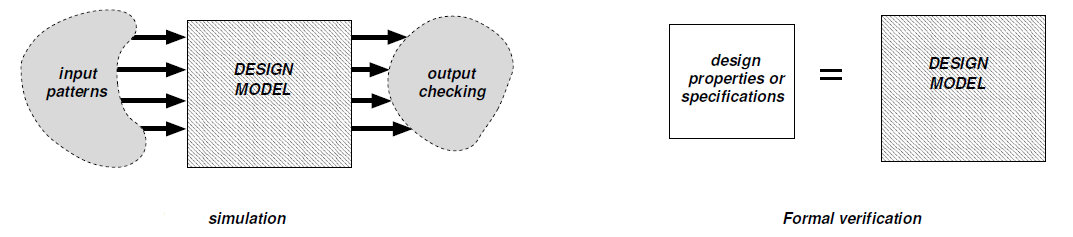
\includegraphics[width=\textwidth]{images/sim_vs_formal.PNG}
	\caption{On the right, a representation of the verification process by Simulation. Stimuli are applied to the DUV inputs and the output behaviour is checked. On the left, Formal Verification checks the DUV against a series of properties that describe the specified behaviour. \cite{thesis-formal}}
	\label{fig:sim-vs-formal}
\end{figure}

The idea of having mathematical proof of the soundness of a design, i.e. the implemented design corresponds to the specification, suggests complex work for the designer, or verification engineer. However, formal verification tools combine three main elements to provide the proof. It comprises proof methods, such as SAT-solving, some specific language, like propositional logic, and models, for example Finite State Machines (FSM). The designer must describe the system as a set of properties and provide them to the tool, which in turn will check if they hold for the RTL implementation. This formal method is also known as property checking. 

Property checking consists of heaving a set of properties describing the specified behaviour of the system and checking whether they can be proved, or checked, for the RTL design.  Therefore, it can be inferred that the RTL description design satisfies the specifications. 

The first step towards having a set of properties is to describe the specified design in an operational view, which can be divided into operations. Each operation represents a specific piece of functional behaviour in finite time interval of the DUV, and can be defined as follows:

\begin{itemize}
    \item Starting important state;
    \item Trigger condition;
    \item Ending important state;
    \item Output behaviour.
\end{itemize}

In other words, an operation describes the behaviour when the design is at a specific important state and a triggering condition happens. Then, the operation defines to which important state the design should go, as well the sequential output behaviour. 

Important states comprise the determination of values for the controls registers of the design. For this reason, they can be also referred as control states. Between the starting state and the ending state, the operation can pass through several non-important states that describe the data path of the design. The triggering condition usually refers to a sequence of inputs, but it can also be a control register having a specific value.

The idea of the operational view is to have a chain of operations that covers the full behaviour of the system. Thus, the end of an operation represents the beginning of other(s). In addition, parallel behaviour can be represented as parallel operations. Examples of operations for a design could be: a read or a write to memory or register file, waiting upon the arrival of a request signal, and the execution of an instruction in a processor.

After specifying the operational view of the design, each operation must be described as a property, or a set of properties, that capture its functionality. In practice, these properties can be written using, for example, System Verilog Assertion (SVA), Property Specification Language (PSL), or even commercial property languages such as ITL \cite{onespin}. A representation of a typical property cab be seen if Fig.~\ref{fig:property}.

\begin{figure}[htb!]
    \begin{lstlisting}
    property accept_request is
    assume:
        at t: state == S1;
        at t: request_i == 1;
    
    prove:
        at t+3: state == S2;
        at t+3: ack_o == 1;
    end property;
    \end{lstlisting}
    \caption{Example of a property that checks the behaviour for a request signal acknowledgement. At an arbitrary time $t$ the circuit is at state $S_1$ and a request signal arrives at the input port $request\_i$. At time $t+3$ the circuit should be at state $S_2$ and an acknowledgement signal is set at the output port $ack\_o$.}
    \label{fig:property}
\end{figure}

The two main parts of a property are the assumptions and commitments. The assumption part characterizes the starting important state and the triggering condition for the operation to be considered. The commitment part depicts the resulting behaviour if the operation is triggered, i.e. outputs description and ending state. A simplified way to represent a property is through a logical implication, Fig.~\ref{fig:a_impl_b}. If a set of assumptions are evaluated as $true$, then the commitments should also be evaluated as $true$ in order to make the property hold. An insight about how verification tools check operational properties is given on Sec.~\ref{subsection:ipc}. Before that, a brief introduction about finite state machines and SAT-solving is presented.

\begin{figure}[htb!]
    \begin{center}
        $a \longrightarrow b$
    \end{center}
    \caption{Logical implication operation where a implies b.}
    \label{fig:a_impl_b}
\end{figure}

\subsection*{Finite State Machine}

A Finite State Machine (FSM) is a deterministic and discrete model of computation that can be, among other applications, used to model a digital circuit. The definition of an FSM is given as follow:

\begin{itemize}
    \item[] $S$: a finite set of states;
    \item[] $s_{0}$: an initial state such that  $s_0 \in S$;
    \item[] $X$: a set of allowed input symbols, input alphabet;
    \item[] $Y$: a set of allowed output symbols, output alphabet;
    \item[] $\delta$: $S \times X \to S$ is a transition function;
    \item[] $\lambda$: $S \times Y \to Y$ is an output function.
\end{itemize}

There are two types of FSM, Mealy and Moore. The aforementioned definition refers to the Mealy type machine. The Moore type only differs on the output function which depends only on the current state $\lambda$: $S \to Y$.

Modelling an electrical circuit as an FSM means that each state of the state machine will correspond to a state of the circuit, i.e. a specific set of values for its control registers. A change of state, determined by the transaction function, and outputs, determined by the output function, will happen upon a change at the inputs. Fig.~\ref{fig:mealy_circuit} depicts a sequential circuit modelled from a Mealy machine.

\begin{figure}[htb!]
	\centering
	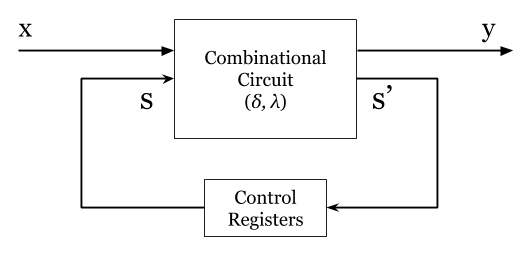
\includegraphics[width=10cm]{images/mealy_circuit.png}
	\caption{Circuit model for a Mealy machine. The combinational circuit models the transition function $\delta$ and output function $\lambda$. The control registers model the state information.}
	\label{fig:mealy_circuit}
\end{figure}

\subsection*{SAT- Solving}

The propositional satisfiability problem, or simply SAT, is the problem of determining if a propositional formula, or Boolean expression, is $satisfiable$, i.e. if it can be evaluated as $true$ for some value combination for its variables. If there is no such combination, and the formula always evaluates to $false$, it is called $unsatisfiable$. 

Considering the formula in Fig.~\ref{fig:a_impl_b}, it is equivalent, and it can be converted, to the formula in the Fig.~\ref{fig:not_a_or_a_and_b}. This expression is $satisfiable$ because it evaluates to $true$ if $a$ is $false$ or if both $a$ and $b$ are $true$. This toy example illustrates how a general property could be converted into a Boolean expression and how SAT-solving could test its satisfiability.

\begin{figure}[htb!]
    \begin{center}
        $\neg a \lor a \land b$
    \end{center}
    \caption{Boolean expression equivalent to logical implication $a \longrightarrow b$.}
    \label{fig:not_a_or_a_and_b}
\end{figure}

\subsection{Interval Property Checking}
\label{subsection:ipc}

Interval Property Checking (IPC) is a formal method to prove an operational property for a design at an arbitrary time interval. Let us consider the sequential circuit in Fig.~\ref{fig:mealy_circuit} and a property that has its starting state at time $t$, and its ending state at time $t+3$, like the one in Fig.~\ref{fig:property}. The sequential circuit could be then converted into combinational by using the unrolling technique, Fig.~\ref{fig:unrolled}. The number of “unrolled circuits” will depend on the time interval of interest. In this case $[t, t+3]$.

\begin{figure}[htb!]
	\centering
	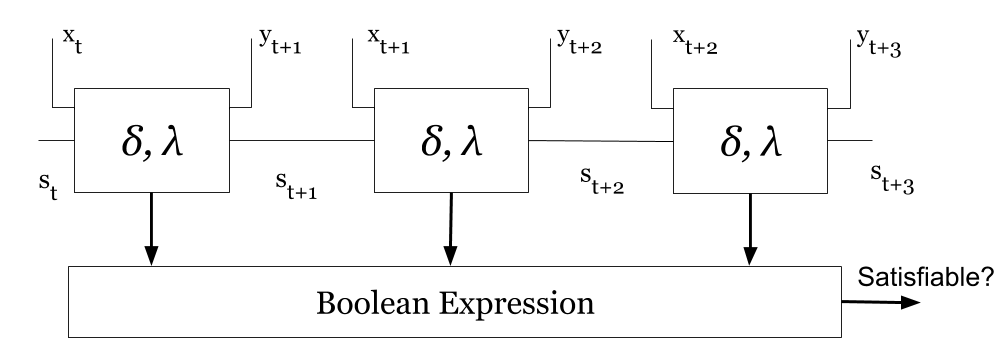
\includegraphics[width=\textwidth]{images/unrolled_circuit.png}
	\caption{Unrolled circuit model for IPC. The unrolled circuit is converted into a Boolean expression which is used to check satisfiability.}
	\label{fig:unrolled}
\end{figure}

The variables from the “unrolled circuit” are then used to describe the property as a Boolean expression. Finally, the SAT-solving tool can evaluate whether the property is $satisfiable$ or not. In other words, IPC proves operational properties by constructing a combinational circuit for the design and solving a SAT problem for it. 

IPC is considered an unbounded model checking method because its time interval of interest can start at an arbitrary time point. It means that it does not start necessarily from the initial state of the circuit. The equivalent Boolean expression for the unbounded circuit from St to St+n is negated so that it cannot evaluate to $true$. If the SAT-solving tool finds a variable combination that evaluates the formula to $true$ it means that a failure was found. In other words, the property holds for the design if the expression is $unsatisfiable$, otherwise, the respective variables combination that make the expression $satisfiable$ are presented by the tool as a counter-example.

Finding a counter-example does not necessarily means that there is a bug in the design. In fact, there could be a fault on the computational model. Since the starting state St can be arbitrary, it is important that it represents a reachable state of the design. During the verification process, when a property fails, the generated counter-example must be analysed in order to identify if it represents a possible scenario for the design of if it is a spurious counter-example, i.e. St represents an unreachable state.

The reachability problem for IPC can be addressed by the concept of invariants. An invariant is a set of states that contains all states reachable from its own states. Let us consider for example a State Machine M. An invariant W of M is any set of states of M that contains all states reachable from W. In this sense, if a property holds for a state St E W, and W contains the initial state, the property holds for every reachable state of the system. Thus, if a spurious counter-example is generated by the tool, reachability information should be added to St as invariants. In practice, the assumptions of the property have to be constrained in order to represent a reachable state. 

\subsection{Gap-free verification}

As previously mentioned, the justification for using Formal Techniques to verify a digital design lies on its potential to achieve completeness. In order to understand this concept better, let us first consider the notion of termination criteria. Conventional verification approaches have their termination criteria relying on the verification plan. Simulation based verification needs a verification plan that will result in a test bench that covers all possible behaviour scenario. This, of course, is very hard to achieve for many designs even using random stimuli techniques. As for assertion-based verification (ABV), the hazard is on determining when the assertions written are enough to comprise the specified behaviour. Formal verification will have its termination criteria anchored on the concept of completeness.

A property set is said to be complete if it has a property, or subset of properties, describing each operation of a design, hence completely describing the specified behaviour of the system. With this, there is no gap between the RTL implementation and specifications, so the name gap-free verification.  

\cite{paper-gapfree} defines a set of operation properties as complete, if it uniquely describes the output behaviour of a circuit according to determination requirements. These determination requirements specify which outputs and states variables are to be determined in each operation. To establish if a set of property is complete, the following completeness tests can be performed \cite{guide-onespin}:

\begin{enumerate}[A.]
    \item \textbf{The Case Split Test:} This test checks whether the chain of operations is comprised by the property set. Therefore, for each state reached by a property, there must be a property starting at this state for every input combination.
    \item \textbf{The Successor Test:} The successor test checks if the chain of properties is uniquely determined. In this sense, for every property the test check if each succeeding property is uniquely determined for its input trace.
    \item \textbf{The Determination Test:} This test will check the determination requirements. It verifies if the outputs and determined state registers, also referred as visible registers, are uniquely determined for all operations.
    \item \textbf{The Reset Property:} The reset test checks the initialization of the design. After the reset sequence, the design should end at a unique important state, and have determined all the signals according to the determination requirements.
\end{enumerate}

\section{Property-Driven Design}

\subsection{SystemC-PPA Model}

\subsubsection{PPA overview}

\subsubsection{SystemC-PPA}

\subsection{The PDD flow}

\subsection{DeSCAM}

\subsection{Completeness with S2QED}


